\documentclass[UTF8]{ctexbook}
\usepackage{polyglossia}
\usepackage{tipa}
\usepackage{multicol}
\usepackage{mdframed}

\setotherlanguages{arabic}
\setotherlanguages{english}

\newfontfamily\arabicfont[Script=Arabic]{MicrosoftSansSerif}
% \newfontfamily\arabicfontit[Script=Arabic]{ZapfinoArabic-Regular}
\newfontfamily\arabicfontit[Script=Arabic]{Rakkas-Regular}
% \newfontfamily\arabicfontit[Script=Arabic]{WaseemLight}
% \newfontfamily\arabicfontit[Script=Arabic]{BArabicStyle}
\newfontfamily\arabicfontbf[Script=Arabic]{DiwanKufi}

\newbool{innote}
\setbool{innote}{false}

\newenvironment{note}{
        \booltrue{innote}  
        \itshape
        % \begin{quote}
        \begin{mdframed}   
    }{
        \boolfalse{innote} 
        \end{mdframed}
        % \end{quote}
    }


\newcommand{\arm}[1]{%
    \ifbool{innote}
        {\textarabic{\arabicfontit{#1}}}  % 在 note 环境中使用斜体
        {\textarabic{#1}}                 % 其他环境使用正常字体
} % 正文中夹杂阿语
% \newcommand{\arm}[1]{\textarabic{#1}}
\newcommand{\ait}[1]{\arabicfontit{#1}}
\newcommand{\abf}[1]{\arabicfontbf{#1}}
\newcommand{\ac}[2]{#2 \hspace{\stretch{1}} \arm{\Large #1}}

\newcommand{\lecon}[1]{\fbox{P#1}} % 对应视频课程P数
\newcommand{\crm}[1]{\textenglish{#1}} % 阿语环境中夹杂中文

\title{\arm{\Huge \arabicfontbf{اَللُّغَةُ الْعَرَبِيَّةُ}} \\ 阿拉伯语笔记}
\author{}
\date{\today}
\begin{document}
\maketitle

\chapter*{前言}

\vfill
\begin{center}

    \arm{\ait {\Large اُطْلُبُوْا العِلْمَ وَلَوْ في الصِّينِ.}}
    
    ~\\

    \emph{求知,哪怕在中国。}
\end{center}
\vfill

\begin{center}
    \begin{center}
        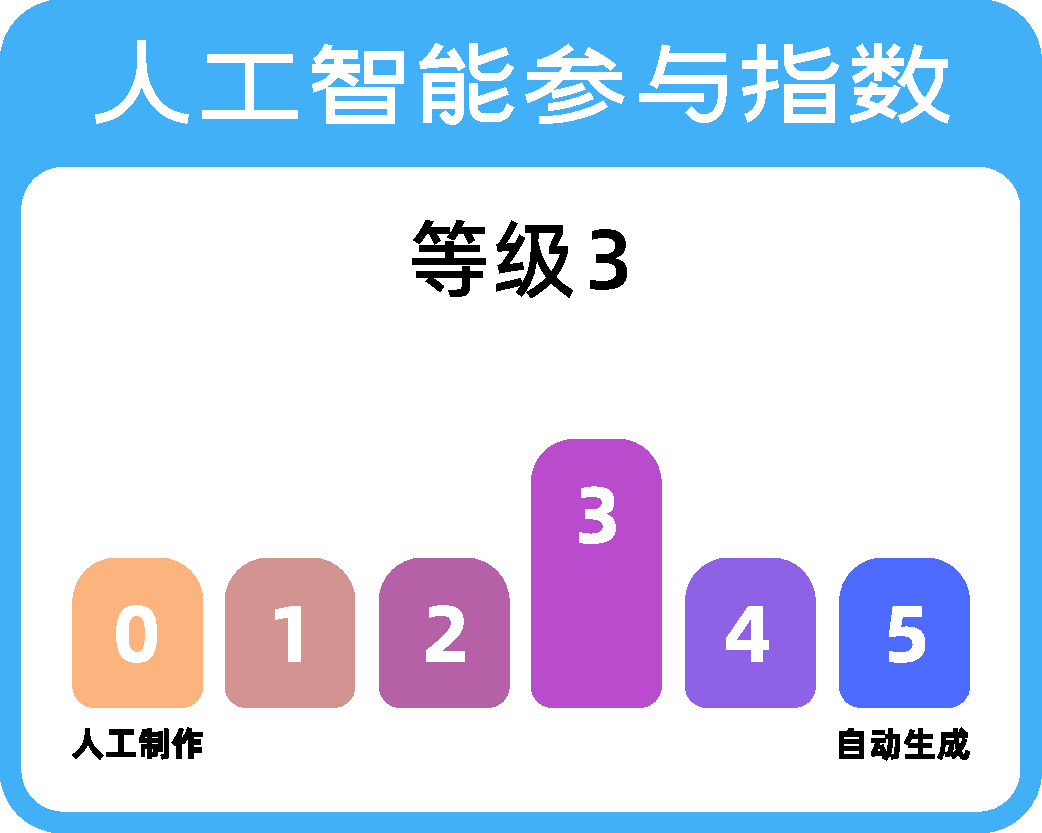
\includegraphics[width=0.4\textwidth]{img/iiia.pdf}
    \end{center}
\end{center}

本笔记借助了GitHub Copilot生成。这玩意太好用了,甚至能猜想到例句(不过发音符号有时会标错),我审核了AI生成的所有内容,但由于毕竟是新接触一套书写系统,难免有拼写疏漏。

\begin{attention}
    这样的格式代表老师在课上强调的知识点。
\end{attention}

\begin{note}
    这样的格式代表我自己的感悟。
\end{note}

\chapter{引言和字母表部分}

本章对应课程P1~P7。

\section{字母表(\arm{اَلْأَبْجَدِيَّةُ الْعَرَبِيَّةُ})及特殊字母写法}

\begin{note}
    字母表请务必跟着视频课学习。笔记只能呈现字母的部分形态。

    此外,在学习阿语字母表时,我愈发意识到,对于老师来说,阿语的一些字形可能已经很熟悉,因此讲解时会快速带过,或干脆略过。但我们来说,面对这样一款陌生的语言,我们需要尝试用最快的速度掌握分辨字形的合适粒度。也就是说,我们需要知道对于这套文字,哪些地方是装饰、哪些地方是区别字母的关键、哪些地方是字体的差异。

    举个例子,\arm{ل} 与 \arm{ا} 搭配而成的 \arm{لا} 有一个独特的词尾型 \arm{ـلا}。在字形呈现上, \arm{لا} 和 \arm{ـلا} 可能很相似,也可能相差很大。这是视频课中没有明确提到的,需要我们自己去观察发现。
\end{note}

\begin{Arabic}
    \begin{tabular}{c|r|r|r|r}
        \crm{独立型} & \crm{读音} & \crm{词头、中、尾连写} & \crm{誊抄} & \crm{特殊形态} \\
        \hline
        أ & أَلِفٌ & أـأـأ & \ait{أـأـأ} & إِ آ \\
        ب & بَاءٌ & بـبـب & \ait{ببب}\\
        ت & تَاءٌ & تـتـت & \ait{تتت} & ة/ـة ةََ \\
        ث & ثَاءٌ & ثـثـث & \ait{ثثث}\\
        ج & جِيمٌ & جـجـج & \ait{ججج}\\
        ح & حَاءٌ & حـحـح & \ait{ححح}\\
        خ & خَاءٌ (厚) & خـخـخ & \ait{خخخ}\\
        د & دَالٌ & دـدـد & \ait{دـدـد}\\
        ذ & ذَالٌ (咬) & ذـذـذ & \ait{ذـذـذ}\\
        ر & رَاءٌ (厚) & رـرـر & \ait{رـرـر}\\
        ز & زَاىٌ & زـزـز & \ait{زـزـز}\\
        س & سِينٌ & سـسـس & \ait{سسس}\\
        ش & شِينٌ & شـشـش & \ait{ششش}\\
        ص & صَادٌ (厚) & صـصـص & \ait{صصص}\\
        ض & ضَادٌ (厚) & ضـضـض & \ait{ضضض}\\
        ط & طَاءٌ (厚) & طـطـط & \ait{تتت}\\
        ظ & ظَاءٌ (厚/咬) & ظـظـظ & \ait{ظـظـظ}\\
        ع & عَينٌ & عـعـع & \ait{ععع}\\
        غ & غَينٌ & غـغـغ & \ait{غغغ}\\
        ف & فَاءٌ & فـفـف & \ait{ففف}\\
        ق & قَافٌ (厚) & قـقـق & \ait{ققق}\\
        ك & كَافٌ & كـكـك & \ait{ككك}\\
        ل & لَامٌ & لـلـل & \ait{للل} & لا/ـلا لاَ لاََ \\
        م & مِيمٌ & مـمـم & \ait{ممم}\\
        ن & نُونٌ & نـنـن & \ait{ننن}\\
        ه & هَاءٌ & هـهـه & \ait{ههه}\\
        و & وَاوٌ & وـوـو & \ait{وـوـو}\\
        ى & يَاءٌ & يـيـى & \ait{ييى}\\
    \end{tabular}
\end{Arabic}

\begin{itemize}
    \item 标``厚''表示其后加 \arm{ـَ} 或 \arm{ـَا} 时发音要更浑厚(靠后,类似\textipa{[A]})。
    \item 标``咬''表示咬舌发音。
    \item \arm{ة} 常位于词尾,一般为阴性名词标志,其前字母永远标 \arm{ـَ} 或 \arm{ـَا} 。\arm{ة} 搭配 \arm{ــََا} 时不写 \arm{ا}。
\end{itemize}

\begin{note}
    在学习满语时我发现,如果过多按照独立型去背诵字母形态,在识读单词的时候会遇到更大的障碍,因为单词中的单词大多数处于词中型。既然如此,为什么不按照词中型将字母整理出来呢?于是,便有了这个列表。

    我根据自己的理解,依照课上的手写体,给每个形状取了名字。此外,请注意阅读顺序(从两边到中间)。
    \begin{itemize}
        \item \ac{ـهـ و ـمـ}{(不规则)h, w, m}
        \item \ac{ـئـ / ـنـ ـتـ ـثـ / ـبـ ـيـ}{(短牙型)' / n, t, th / b, y}
        \item \ac{ـلـ ـكـ}{(长牙型)l, k}
        \item \ac{ـــحـ / ـــخـ / ـــجـ}{(闪电型)ḥ / kh / \textipa{\textdyoghlig}}
        \item \ac{د ذ / ر ز}{(小钩型)d, dh / r, z}
        \item \ac{ـسـ ـشـ}{(横线型)s, sh}
        \item \ac{ـفـ ـقـ / ـطـ ـظـ / ـصـ ـضـ}{(上圈型)f, q / ṭ, ẓ / ṣ, ḍ}
        \item \ac{ـعـ ـغـ}{(三角型)`, gh}
    \end{itemize}

    可以看到,转写中为拉丁字母加点,对应到阿文很可能会完全变成另一个字母。于是,我又整理了如下表格,来表示部分字母的发音关系。该表中,关于中心轴对称的辅音互为清浊关系。越远离中心轴,表示发音越难(加喉音、加顶音等)。对应转写并列展示。

    \begin{center}
    \begin{multicols}{2}
    \begin{tabular}{cc||cc}
        \hline
        \arm{ض} & \arm{د} & \arm{ت} & \arm{ط} \\
        && \arm{ك} & \arm{ق} \\
        & \arm{غ} & \arm{خ} \\
        \arm{ع} && \arm{ه} & \arm{ح}\\
        & \arm{ج} & \arm{ش} \\
        & \arm{ز} & \arm{س} & \arm{ص} \\
        \arm{ظ} & \arm{ذ} & \arm{ث} \\
        \hline
    \end{tabular}

    \begin{tabular}{cc||cc}
    
        \hline
        ḍ & d & t & ṭ \\
        && k & q \\
        & gh & kh \\
        ` && h & ḥ \\
        & \textipa{\textdyoghlig} & sh \\
        & z & s & ṣ \\
        ẓ & dh & th \\
        \hline

    \end{tabular}
    \end{multicols}
    \end{center}
\end{note}

\section{单词和课文}

\subsection{引入和字母部分}

\begin{itemize}
    \item \ac{اَلْعَرَبِيَّةُ}{阿拉伯语}
    \item \ac{اَلْبُلْدَانُ الْعَرَبِيَّةُ}{阿拉伯国家}
    \item \ac{صَحْرَاءُ}{沙漠}
    \item \ac{اَصَّحْرَاءُ الْكُبْرَى}{撒哈拉沙漠(沙漠--最大的)}
    \item \ac{جَمَلٌ}{骆驼}
    \item \ac{نِفْطٌ}{石油}
    \item \ac{بِتْرُولٌ}{石油(音译自petrol)}
    \item \ac{قَهْوَةٌ}{咖啡}
    \item \ac{أَلْفُ لَيْلَةِِ وَلَيْلَةٌ}{《一千零一夜》(一千--夜(属)--和一夜)}
    \item \ac{جُبْرَانُ}{纪伯伦}
    \item \ac{اَللُّغَاتُ السَّامِيَّةُ}{闪米特语族(Semitic Languages)}

\end{itemize}

\section{语法}

阿拉伯语属于闪含语系闪语族(闪米特语族),诞生于阿拉伯半岛,最早的文献可以追溯到公元6世纪阿拉伯半岛北部的石刻。

阿拉伯语辅音相对复杂,一般三个辅音字母构成基本含义。例如:

\begin{itemize}
    \item \ac{فَهِمَ}{理解}
    \item \ac{أَفِهَمَ}{使……理解}
    \item \ac{تَفَاهَمَ}{相互理解}
    \item \ac{اِسْتَفْهَمَ}{询问(要求理解)}
    \item \ac{مَفْهُومٌ}{概念(被理解的事物)}
\end{itemize}

阿拉伯语有名词、动词、虚词,没有系动词:

\begin{itemize}
    \item \ac{هَذَا كِتَابٌ.}{这--一本书。(\arm{هَذَا}注音为\arm{هَاذَا})}
\end{itemize}

阿语动词常在句首:遇到--张三(主格)--李四(宾格)

\chapter{hello, world}

\lecon{8.1}

\section{单词和课文}

\begin{itemize}
    \item \ac{أَهْلٌ}{家人}
    \item \ac{وَـ}{和--}
    \item \ac{سَهْلٌ}{平原}
    \item \ac{مَنْ}{谁}
    \item \ac{أَنْتَ / أَنْتِ}{你}
    \item \ac{أَنَا}{我}
    \item \ac{هُوَ / هِىَ}{他}
\end{itemize}

\begin{Arabic}
    - أَهْلاََ وَسَهْلاََ!

    - أَهْلاََ وَسَهْلاََ!

    - مَنْ أَنْتَ؟

    - أَنَا مَنْصُورٌ، وَمَنْ أَنْتِ؟

    - أَنَا يُمْنَى.

    - مَنْ هُوَ؟

    - هُوَ أَحْمَدُ.

    - وَمَنْ هِىَ؟

    - هِىَ يُمْنَى.
\end{Arabic}

\section{语法}

\subsection{\lecon{8.3} \arm{ن} 的显读( \arm{أَلْإِظْهَارُ})}

\arm{ن} 在以下字母前面发音明显:\arm{أ ه ح خ ع غ}

\begin{itemize}
    \item \ac{أَنْحَاءٌ}{}
    \item \ac{أَنْخَابٌ}{}
    \item \ac{صَنْعَاءٌ}{萨那(也门首都)}
    \item \ac{أَنْغَاءٌ}{}
\end{itemize}

\subsection{\lecon{8.4} 词法}

阿语有三种词性。

\begin{itemize}
    \item 动词
    \begin{itemize}
        \item 人称:1/2/3
        \item 性:阴/阳
        \item 数:单/双/复
        \item 格:主/宾/切
        \item 时式:过去/现在/命令
    \end{itemize}
    \item 名词
    \begin{itemize}
        \item 性:阴/阳
        \item 数:单/双/复
        \item 格:主/宾/属
        \item 式:泛指/确指
    \end{itemize}
    \item 虚词
    \begin{itemize}
        \item 介词(需要加名词属格)
        \item 联词
        \item 疑问虚词、应答虚词
        \item …………
    \end{itemize}
\end{itemize}

阿语句子分为以动词开头的动词句和以名词开头的名词句。
\chapter{君の名は?}

\lecon{9.1}

\section{单词和课文}

\begin{itemize}
    \item \ac{مَا}{谁}
    \item \ac{اِسْمٌ}{名字}
    \item \ac{اِسْمُكَ / اِسْمُكِ}{你的名字}
    \item \ac{اِسْمِى}{我的名字}
    \item \ac{اِسْمُهُ / اِسْمُهَا}{他的名字}
    \item \ac{بِ}{prep. 借助}
    \item \ac{أَهْلََا بِكَ!}{你好}
    \item \ac{حَسَنََا}{好的}
    \item \ac{إِلَى}{prep. 向、到}
    \item \ac{اَلْ}{冠词(无\arm{ء
    })}
    \item \ac{لِقَاءٌ}{n. 见面}
    \item \ac{إِلَى اللِّقَاءِ}{再见}
\end{itemize}

\begin{Arabic}
    - أَهْلاََ وَسَهْلاََ! 

    - أَهْلاََ وَسَهْلاََ!

    - مَا اسْمُكَ؟

    - اِسْمِى أَهْمَدُ. وَمَا اسْمُكَ؟

    - اِسْمِى مَنْصُورٌ.

    - أَهْلاََ وَسَهْلاََ!

    - أَهْلاََ بِكَ!

    - أَنَا مَنْصُورٌ. وَمَا اسْمُكِ؟

    - اِسْمِى يُمْنَى.

    - حَسَنََا.إِلَى للِّقَاءِ!

    - إِلَى للِّقَاءِ! 
\end{Arabic}

\begin{note}
    \arm{مَا اسْمُكَ؟}读音为\arm{مَسْمُكَ}。

    \arm{إِلَى} (介词)后面 \arm{لِقَاءٌ} 变为属格 \arm{لِقَاءِ} 。
\end{note}
\chapter{我是学生}

\lecon{10.1}

\section{单词和课文}

\begin{itemize}
    \item \ac{هَلْ}{……吗?}
    \item \ac{طَالِبٌ / طَلِبَةٌ}{学生}
    \item \ac{طَبِيبٌ / طَبِيبَةٌ}{医生}
    \item \ac{صَدِيقٌ / صَدِيقَةٌ}{朋友}
    \item \ac{صَدِيقِى / صَدِيقَتِى}{我的朋友}
    \item \ac{زَمِيلٌ / زَمِيلَةٌ}{同学/同事}
    \item \ac{زَمِيلِى / زَمِيلَتِى}{我的同学/同事}
    \item \ac{يَا}{喂(后面人名末尾的 \arm{ـٌ} 变成 \arm{ـُ})}
    \item \ac{نَعَمْ}{是}
    \item \ac{لَا}{否}
    \item \ac{مُدَرِّسٌ / مُدِرِّسَةٌ}{老师}
    \item \ac{مُهَنْدِسٌ / مُهَنْدِسَةٌ}{工程师}
    \item \ac{مُمَرِّضٌ / مُمَرِّضَةٌ}{护士}
\end{itemize}

\begin{Arabic}
    - أَهْلاََ وَسَهْلاََ!

    - أَهْلاََ بِكَ!

    - هَلْ أنْتَ طَالِبٌ؟

    - نَعَمْ. أَنَا طَالِبٌ. هَلْ أَنْتِ طَالِبَةٌ أَيْضََا؟

    - لَا، أَنَا طَبِيبَةٌ.

    - يَا يُمْنَى، هُوَ صَدِيقِى، اِسْمُهُ أَحّمَدُ.

    - أَهْلاََ بِكَ، يَا أَحّمَدُ

    - أَهْلاََ بِكِ!

    - هَلْ أَنْتَ طَالِبٌ أَيْضََا؟

    - نَعَمْ. أَنَا طَالِبٌ أَيْضََا. أَنَا زَهِيلُهُ.

    - نَعَمْ، هُوَ زَمِيلِى.
\end{Arabic}

\begin{note}
    \arm{أَيْضا} 也,\arm{زَمِيلُهُ} 他的同学。
\end{note}

\section{语法}

\subsection{\lecon{10.2} ……的……}

\begin{note}
    这是属格接尾人称代词的先导。
\end{note}

以 \arm{زَمِيلٌ / زَمِيلَةٌ} 为例。

\begin{center}
    \begin{Arabic}
    \begin{tabular}{r|c|rr}
         & \crm{变位方式} & 阳 & 阴 \\
        \hline
        \crm{原型} & & زَمِيلٌ & زَمِيلَةٌ \\
        أَنَا & ـٌ $\leftarrow$  ـِى  & زَمِيلِى & زَمِيلَتِى \\
        أَنْتَ &   &  &  \\
        أَنْتِ &  &  &  \\
        هُوَ & ـٌ $\leftarrow$ ـُهُ & زَمِيلُهُ & زَمِيلَتُهُ \\
        هِيَ & ـٌ $\leftarrow$ ـُهَا & زَمِيلُهَا & زَمِيلَتُهَا \\
    \end{tabular}
\end{Arabic}
\end{center}


\subsection{\lecon{10.3} 名词双数}

主格:\arm{ـٌ} \cto \arm{ـَانِ}

宾格、属格:\arm{ـٌ} \cto \arm{ـَيْنِ}

\begin{center}
    \begin{tabular}{cc|cc}
        两个…… & & 主格 & 宾、属格 \\
        \hline
        房子 & \arm{بَيْتٌ} & \arm{بَيْتَانِ} & \arm{بَيْتَِيْنِ} \\
        男人 & \arm{رَجُلٌ} & \arm{رَجُلَانِ} & \arm{رَجُلَيْنِ} \\
        小伙子 & \arm{فَتََى} & \arm{فَتَيَانِ} & \arm{فَتَيَيْنِ} \\
        姑娘 & \arm{فَتَاةٌ} & \arm{فَتَاتَانِ} & \arm{فَتَاتَيْنِ} \\
        公司 & \arm{شَرِكَةٌ} & \arm{شَركَتَانِ} & \arm{شَركَتَيْنِ} \\
    \end{tabular}
\end{center}

所谓``弄假成真'',即诸如 \arm{فَتََى}末尾 \arm{ى}形的 \arm{أ}直接作为 \arm{ى}而处理成 \arm{ـيـ}。

\subsection{\lecon{10.4} 主格独立人称代词}

\begin{center}
    \begin{Arabic}
    \begin{tabular}{c|c|c|c}
        \crm{人称} & \crm{单数} & \crm{双数} & \crm{复数} \\
        \hline
        \crm{一} & أَنَا = أَنَا & \crm{无} & نَحْنُ = نَحْنُ \\
        \crm{二} & أَنْتَ / أَنْتِ & أَنْتُمَا = أَنْتُمَا & أَنْتُمْ / أَنْتُنَّ \\
        \crm{三} & هُوَ / هِيَ & هُمَا = هُمَا & هُمْ / هُنَّ 
    \end{tabular}
\end{Arabic}
\end{center}

\subsection{\lecon{10.5}属格接尾人称代词}

\begin{itemize}
    \item \ac{مِنْ}{prep. 来自}
    \item \ac{عَلَى}{在……上}
\end{itemize}

不独立使用,后缀与名词词尾。后缀变位:

\begin{center}
    \begin{Arabic}
        \begin{tabular}{c|c|c|c}
            \crm{人称} & \crm{单数} & \crm{双数} & \crm{复数} \\
            \hline
            \crm{一} & أَنَا : ـِى  & \crm{无} & نَحْنُ : ـنَا \\
            \hline
            \multirow{2}{*}{\crm{二}} & أَنْتَ : ـكَ & \multirow{2}{*}{أَنْتُمَا : ـكُمَا} & أَنْتُمْ : ـكُمْ \\
                & أَنْتِ : ـكِ & & أَنْتُنَّ : ـكُنَّ \\

            \hline
            \multirow{2}{*}{\crm{三}} & هُوَ : ـهُ & \multirow{2}{*}{هُمَا : ـهُمَا} & هُمْ : ـهُمْ \\
                & هِىَ : ـهَا & & هُنَّ : ـهُنَّ \\
        \end{tabular}
    \end{Arabic}
\end{center}

\begin{note}
    不知道为什么,课上喜欢从更为复杂的第三人称开始,讲到较为简单的第一人称。但笔记仍然遵循一、二、三人称的顺序了。

    具体来说,第三人称比较好记,双、复数完全就是直接把独立主格人称代词放到后面,单数却是一个短音一个长音。

    如果说第三人称的主题是 \arm{ه},那第二人称的主题就是 \arm{ك}。懂满语的人看到这直接就笑出来了:双、复数直接就是``去掉第三人称的圈''。

    单数和第一人称硬记。

    属格不改变原词的性。如 \arm{بَيْتٌ}(阳性)接阴性后缀后(如 \arm{بَيْتُكِ})仍为阳性。
\end{note}

\paragraph{鼻音符不能接属格接尾人称代词} 去掉 \arm{ـََ، ـِِ، ـٌ}的双写,或直接被第一人称单数的 \arm{ـِى}替代。

\paragraph{冠词和属格接尾人称代词不能同时存在} 很好理解,ma maison可以但la ma maison不可以。

\paragraph{第三人称音变} 以下结尾的名词变第三人称属格时 \arm{ـهُ/ـهُـ}变 \arm{ـهِ/ـهِـ}:

\begin{Arabic}
    \begin{itemize}
        \item ـِ
        \item ـِى
        \item ـَىْ
    \end{itemize}
\end{Arabic}

以 \arm{بَيْتٌ}的词组 \arm{فِي بَيْتِ}(在房子里)为例:

\begin{center}
    \begin{Arabic}
        \begin{tabular}{c|c|c|c}
            \crm{在房子里} & \crm{第三人称单数} & \crm{第三人称双数} & \crm{第三人称复数} \\
            \hline
            \multirow{2}{*}{فِي بَيْتِ} & هُوَ : فِي بَيْتِهِ & \multirow{2}{*}{هُمَا : فِي بَيْتِهِمَا} & هُمْ : فِي بَيْتِهِمْ \\
                & هِىَ : فِي بَيْتِهَا & & هُنَّ : فِي بَيْتِهِنَّ \\
        \end{tabular}
    \end{Arabic}
\end{center}

\begin{note}
    其实就是 ``真[i]'' (而不含 \arm{ى}形 \arm{ا}这样的``假[i]'')结尾,真的很像元音和谐律。
\end{note}

\paragraph{附加的 \arm{ن}接属格接尾人称代词要去掉} 例如名词双数、阳性完整式复数的情况。

\begin{note}
    记得连着 \arm{ن}的元音一期去掉,即去掉整个音节。
\end{note}

\begin{center}

\begin{tikzpicture}[
    scale=3,              % 图形缩放比例
    every node/.style={}, % 所有节点字体大小
    vertex/.style={circle, fill=black, inner sep=1.5pt}, % 顶点样式
    edge label/.style={midway, fill=white, inner sep=1pt}, % 边注释样式
]

% 定义正方体顶点坐标(三维坐标:x, y, z)
\coordinate (A) at (0,0,0);
\coordinate (B) at (-1,0,0);
\coordinate (C) at (-1,-1,0);
\coordinate (D) at (0,-1,0);
\coordinate (E) at (0,0,-1);
\coordinate (F) at (-1,0,-1);
\coordinate (G) at (-1,-1,-1);
\coordinate (H) at (0,-1,-1);

\draw (A) node[vertex, label=below right:\arm{بَيْتٌ}{\footnotesize 房}] {};
\draw (B) node[vertex, label=left:{\footnotesize 俩房} \arm{بَيْتَانِ}] {};
\draw (D) node[vertex, label=right:\arm{بَيْتُهُ}{\footnotesize 他的房}] {};
\draw (C) node[vertex, label=left:{\footnotesize 他的俩房} \arm{بَيْتَاهُ}] {};

\draw (E) node[vertex, label=right:\arm{فِى بَيْتِِ}{\footnotesize 房里}] {};
\draw (F) node[vertex, label=left:{\footnotesize 俩房里} \arm{فِى بَيْتَيْنِ}] {};
\draw (H) node[vertex, label=right:{\footnotesize 他房里}\arm{فِى بَيْتِهِ}] {};
\draw (G) node[vertex, label=below:{\footnotesize 他的俩房里} \arm{فِى بَيْتَيْهِ}] {};

\draw[thick] (C) -- (D);
\draw[thick, dashed] (E) -- (F);
\draw[thick, dashed] (G) -- (H);
\draw[thick, dashed] (H) -- (E);

\draw[thick, -{Stealth[length=3mm]}] (B) -- (C) node[edge label, sloped, right, rotate=180]{\footnotesize (去 \arm{ن})};
\draw[thick, -{Stealth[length=3mm]}, dashed] (F) -- (G)node[edge label, sloped, left, rotate=180]{\footnotesize (去 \arm{ن})};

\draw[thick, -{Stealth[length=3mm]}] (A) -- (B) node[edge label]{双};
\draw[thick, -{Stealth[length=3mm]}] (A) -- (D) node[edge label, sloped, rotate=180]{属他};
\draw[thick, -{Stealth[length=3mm]}, dashed] (A) -- (E) node[edge label, sloped]{宾};

\end{tikzpicture}

\end{center}

\begin{note}
    \arm{بَيْتٌ} \cto 宾格泛指 \arm{فِى بَيْتِِ},加属格接尾人称代词``在他的房子里''步骤如下:
    \begin{enumerate}
        \item 结尾不能鼻音符:\arm{فِى بَيْتِِ} \cto \arm{فِى بَيْتِ};
        \item \arm{ـِ}结尾,\arm{ـهُ}变 \arm{ـهِ}:\arm{فِى بَيْتِهُ} \cto \arm{فِى بَيْتِهِ}。
    \end{enumerate}
\end{note}

(还没学到)再如,完整式阳性复数加接尾人称代词:

\begin{itemize}
    \item 主格: \arm{ـُونَ} \cto \arm{ـُوـ..}
    \item 宾属格: \arm{ـِينَ}  \cto \arm{ـِيـ..}
\end{itemize}

\begin{Arabic}
    \begin{center}
        \begin{tabular}{c|cc}
            \crm{老师} & \crm{老师们} & \crm{她的老师们} \\
            \hline
            مُدَرِّسٌ & مُدَرِّسُونَ & مُدَرِّسُوهَا \\
             & مِنْ مُدَرِّسِينَ & مِنْ مُدَرِّسِيهَا
        \end{tabular}
    \end{center}
\end{Arabic}



\paragraph{第一人称读法变化} ``我的''接在下列词尾后时,不吞掉原词尾,直接加 \arm{ـىَ}

\begin{Arabic}
    \begin{itemize}
        \item ـَا
        \item ـُو
        \item ـَى
    \end{itemize}
\end{Arabic}

\begin{itemize}
    \item \ac{بَيْتَانِ \ato بَيْتَاىَ \ato عَلَى بَيْتَيْىَ}{俩房 \cto 我的俩房 \cto 我的俩房上}
    \begin{itemize}
        \item 第一个变化是先去 \arm{ن}再由于 \arm{ـتَا}而接 \arm{ـىَ}
        \item 第二个变化是先去 \arm{ن}再由于 \arm{ـتَىْ}而接 \arm{ـىَ}
    \end{itemize}
    \item \ac{مُدَرِّسُونَ \ato مُدَرِّسُوىَ \ato مِنْ مُدَرِّسِيىَ}{老师们 \cto 我老师们  \cto 来自我的老师们 \\}
\end{itemize}


在以下介词后时,也有读音变化:

\begin{itemize}
    \item \ac{بِ \ato بِيَ}{凭借、在 \cto 凭借我、在我这}
    \item \ac{فِي \ato فِيَّ}{在……里 \cto 在我的里面}
    \item \ac{مِنْ \ato مِنِّي}{从 \cto 从我这}
    \item \ac{عَنْ \ato عَنِّي}{关于、通过 \cto 关于我、通过我}
\end{itemize}

\begin{note}
    注意,指的是在两个介词后面直接变位(如``凭借我'')。此外,\arm{فِي}和变音后缀的 \arm{ـنِي}的长音下面是加两点的,不知道为什么。

    此外,我是真没想到介词也能这么变。
\end{note}

\chapter{卧槽,学霸!}

\section{\lecon{12.2} 单词和课文}

\begin{itemize}
    \item \ac{كَيْفَ}{n. 怎么样}
    \item \ac{حَالٌ}{情况}
    \item \ac{خَيْرٌ}{最好的}
    \item \ac{بِخَيْرٍ}{……很好(\arm{بِـ} 后属格,因此是 \arm{ـٍ})}
    \item \ac{شُكْرًا}{谢谢}
    \item \ac{قَلَمٌ جـ أَقْلَامٌ}{笔}
    \item \ac{مِقْلَمَةٌ جـ مَقَالِمُ}{笔袋}
    \item \ac{كِتَابٌ جـ كُتُبٌ}{书}
    \item \ac{دِرَاسَةٌ}{n. 学习(表抽象意义的词根形式)}
    \item \ac{لِمَنْ ...؟}{……是谁的?}
    \item \ac{... لِي.}{……是我的。}
    \item \ac{يَالَكَ مِنْ ...!}{你真是个……的人啊!}
    \item \ac{مُجْتَهِدٌ فِي ...}{在……上努力的人}
    \item \ac{بَابٌ جـ أَبْوَابٌ}{m. 门}
    \item \ac{نَافِذَةٌ جـ نَوَافِذُ}{f. 窗}
    \item \ac{مَكْتَبٌ جـ مَكَايِبُ}{m. 课桌}
    \item \ac{كُرْسِيٌّ جـ كَرَاسٍ }{(缺尾)m. 椅}
    \item \ac{اِسْمٌ جـ أَسْمَءٌ}{名字}
\end{itemize}

\begin{attention}
    \arm{جـ} 表示后侧是前侧的破碎式复数。

    书等指物名词复数语法上当成阴性单数看待。

    \begin{Arabic}
        \begin{itemize}
            \item هَزِهِ أَبْوَابٌ.
        \end{itemize}
    \end{Arabic}

    复数的 \arm{كَرَاسٍ} 为所谓``缺尾名词'',即其词尾永远是 \arm{ـٍ},并不代表它是属格。
\end{attention}

\begin{note}
    似乎只有破碎式复数而没有``破碎式双数''?
    \begin{itemize}
        \item \ac{هَزَانِ بَابَانِ.}{这是两扇门。}
    \end{itemize}
\end{note}

\begin{Arabic}
    - أَهْلًا وَسَهْلًا!

    - أَهْلًا بِكَ.

    - كَيْفَ حَالُكَ؟

    - أَنَا بِخَيْرٍ، شُكْرًا. وَأَنْتَ؟

    - أَنَا بِخَيْرٍ.

    - مَا هَزَا؟

    - هَزَا قَلَمٌ.

    - وَ مَا هَزِهِ؟

    - هَزِهِ مِقْلَمَةٌ.

    - وَ مَا هَزَا؟

    - هَزَا كِتَابٌ.

    - وَمَا هَزِهِ؟

    - هَزِهِ كُتُبٌ.

    - لِمَنْ هَزِهِ الْكُتُبُ؟

    - هَزِهِ الْكُتُبُ لِي.

    - يَا لَكِ مِنْ مُجْتَهِدَةٍ فِي الدِّرَاسَةِ!
\end{Arabic}

\paragraph{某物是谁的?} \arm{لِـ}--疑问代词(此课只有 \arm{لِمَنْ})+指示代词+ \arm{الـ}--物(注意词尾 \arm{ـٌ} 改成 \arm{ـُ})。

\paragraph{某物是……的} 指示代词+ \arm{الـ}--物+ \arm{لِـ}--属格接尾人称代词。

\begin{Arabic}
    \begin{itemize}
        \item هَزَا الْقَلَمُ / هَزِهِ الْمِقْلَمَةُ ...
        \begin{itemize}[label=\crm{--}]
            \item لِي
            \item لَكَ
            \item لَكِ
            \item لَهُ
            \item لَهَا
        \end{itemize}
    \end{itemize}
\end{Arabic}

\paragraph{你真是……的人啊!}  两种说法:

\begin{itemize}
    \item 感叹虚词+ \arm{لِـ}--人称代词 + \arm{مِنْ} + 名词\emph{属格泛指}。
    \item 感叹虚词+ \arm{لِـ}--人称代词 + 名词\emph{宾格泛指}。
\end{itemize}

\begin{Arabic}
    \begin{itemize}
        \item يَا لَكَ مِنْ رَجُلٍ! = يَا لَكَ رَجُلًا!
        \item يَا لَكَ مِنْ مُجْتَهِدٍ فِي الدِّرَاسَةِ! = يَا لَكَ مُجْتَهِدًا فِي الدِّرَاسَةِ!
    \end{itemize}
\end{Arabic}

\section{语法}

\subsection{\lecon{12.3} 泛指和确指}

\begin{note}
    没什么好记的,同直觉一致。
\end{note}

\subsection{\lecon{12.4} 冠词的发音}

\begin{Arabic}
    \begin{center}
        \begin{tabular}{c|cc}
            & ا & ل \\
            \hline
            \crm{发音} & \crm{前面没有东西}  & \crm{后面是太阴字母} \\
            \crm{不发音} & \crm{前面有东西} & \crm{后面是太阳字母}\\
        \end{tabular}
    \end{center} 
\end{Arabic}

\arm{ل} 不发音时,后面的太阳字母读叠音。

太阴字母:\arm{أ ب ج ح خ ع غ ف ق ك م ه و ى}

太阳字母:\arm{ت ث د ذ ر ز س ش ص ض ط ث ل ن}

\begin{note}
    太阴/太阳字母和前面冠词的 \arm{ل} 是否发音似乎是最讨厌的循环定义。不过,可以从字形上来简单记忆:

    \begin{center}
    \begin{tabular}{c|cc}
        & 太阴/ \arm{لْ} 发音 & 太阳/叠音+ \arm{ل} 不发音 \\
        \hline
        不规则 & 全部 & 无 \\
        短牙型 & 其他(带 \arm{ء}、下面带点) & 上面加点 \\
        长牙型 & 带 \arm{ء} 的 & 其他(\arm{ل}) \\
        闪电型 & 全部 & 无 \\
        小钩型 & 无 & 全部 \\
        横线型 & 无 & 全部 \\
        上圈型 & 只有圈点的 & 圈上带杠、牙的 \\
        三角型 & 全部 & 无
    \end{tabular}
    \end{center}

    即:

    \begin{center}
    \begin{tabular}{c|cc}
        & 太阴/ \arm{لْ} 发音 & 太阳/叠音+ \arm{ل} 不发音 \\
        \hline
        不规则 & \arm{ه و م} & \arm{} \\
        短牙型 & \arm{ـئـبـيـ} & \arm{ـنـتـثـ} \\
        长牙型 & \arm{ك} & \arm{ل} \\
        闪电型 & \arm{ـجـحـخـ} & \arm{} \\
        小钩型 & \arm{} & \arm{دذرز} \\
        横线型 & \arm{} & \arm{ـسـشـ} \\
        上圈型 & \arm{ـفـقـ} & \arm{ـصـضـطـظـ} \\
        三角型 & \arm{ـغـعـ} & \arm{} 
    \end{tabular}
    \end{center}
\end{note}

\subsection{\lecon{12.5} 名词的破碎式复数}

一些变尾名词的破碎式复数是半变尾名词。

\begin{itemize}
    \item \ac{زَمِيلٌ جـ زُمَلَاءُ}{同学}
    \item \ac{طَبِيبٌ جـ أَطِبَّاءُ}{医生}
    \item \ac{صَدِيقٌ جـ أَصْدِقَاءُ}{朋友}
\end{itemize}

\begin{note}
    课中有说半变尾名词意味着 \arm{زُمَلَاءُ}、\arm{أَطِبَّاءُ}、\arm{أَصْدِقَاءُ} 的宾、属格分别为 \arm{زُمَلَاءَ}、 \arm{أَطِبَّاءَ}、 \arm{أَصْدِقَاءَ}。没说为啥。
\end{note}

一些指人的阳性名词,破碎式复数带有 \arm{ة},但仍为阳性。

\begin{itemize}
    \item \ac{أُسْتَاذٌ جـ أَسَاتِذَةٌ}{教授}
    \item \ac{طَالِبٌ جـ طَلَبَةٌ}{学生}
\end{itemize}

一些名词有多种破碎式复数。

\begin{Arabic}
    \begin{itemize}
        \item طَالِبٌ جـ طَلَبَةٌ \& طُلَّابٌ
    \end{itemize}
\end{Arabic}

一些外来词的复数也是破碎的。

\begin{itemize}
    \item \ac{بَنْكٌ جـ بُنُوكٌ}{银行}
    \item \ac{فِلْمٌ جـ أَفْلَامٌ}{电影}
    \item \ac{قَيْصَرٌ جـ قَيَاصِرَةٌ}{凯撒/沙皇}
\end{itemize}

\begin{note}
    对于总结规律记忆破碎式复数,课上举了两组例子,抄录如下。
    \begin{Arabic}
        \begin{itemize}
            \item ـ ـ ـ جـ أَـْ ـَاـٌ
            \begin{itemize}[label=\crm{--}]
                \item فِلْمٌ جـ أَفْلَامٌ
                \item قَلَمٌ جـ أَقْلَامٌ
                \item اِسْمٌ جـ أَسْمَءٌ
            \end{itemize}
            \item ـ ـْ ـَ ـٌ جـ ـَ ـَاـِ ـَةٌ
            \begin{itemize}[label=\crm{--}]
                \item أُسْتَاذٌ جـ أَسَاتِذَةٌ
                \item قَيْصَرٌ جـ قَيَاصِرَةٌ
            \end{itemize}
        \end{itemize}
    \end{Arabic}
\end{note}

\subsection{\lecon{12.6} 名词句}

词首是名词就是名词句,判断句首时忽略某些虚词。

名词句的两个最基本的要素:

\begin{description}
    \item[起语] 就是接は的那东西。主格,确指;倒装名词句中为泛指。
    \item[述语] 就是接です的东西。主格,尽量泛指;意义上不能泛指也可以确指。
\end{description}

上述的主格指的是处于主格的地位,因为有时无法从变位看出具体的格。记得适当的时候性数配合。

\begin{note}
    俩都是主格。
\end{note}

\begin{itemize}
    \item \ac{أَنَا بِخَيْرٍ.}{我很好。}
    \item \ac{هَذِهِ الْكُتُبُ لِي.}{这些书是我的。}
    \item \ac{هِيَ جَمِيلَةٌ.}{她美丽。}
\end{itemize}

介词短语 \arm{بِخَيْرٍ}、 \arm{لِي} 看不出格位,但处于主格地位。半主动名词 \arm{جَمِيلَةٌ} 当形容词来用。

\end{document}